\documentclass[11pt]{report}
\usepackage{amsmath}
\usepackage{algorithm}
\usepackage[noend]{algpseudocode}
\usepackage[margin=1.5in]{geometry}
\usepackage{amsfonts}
\usepackage{graphicx}
\usepackage{epstopdf}
\usepackage[mathscr]{euscript}
\makeatletter
% Reinsert missing \algbackskip
\def\algbackskip{\hskip-\ALG@thistlm}
\makeatother

\begin{document}
	
	\chapter{Overview on Machine Learning Applied to Satellite Communications}
	\par \textbf{\textit{make table of acronyms for overall report}}
	\par In this chapter, an overview of the SCaN Testbed Cognitive Engine will be provided. In order to understand and motivate decisions that were made in the initial development, a general overview about machine learning will first be provided. Then, the work accomplished by the team prior to this thesis will be described. After this, topics that are relevant to the improvements introduced to the CE by this thesis will be discussed. Finally, a summary of the chapter will be provided.
	\section{A General Overview of Machine Learning}
	\par With the advent of increasingly more capable and accessible processors, machine learning has become a useful tool in many different fields. This is in part driven by the flexibility and efficiency that machine learning is capable of. There are three major categories of ML algorithms\cite{IntroductionToML}: supervised learning, unsupervised learning, and reinforcement learning. Supervised learning takes a set of input values $X$ and a set of target results $Y$, and attempts to create a mapping $x \to g(x)\to y$. Once the algorithm is trained, this mapping $g(x)$ can be used with new input values $x_{new}$ to predict new target values $y_{new}$. Unlike supervised learning, unsupervised learning is only given a set of input values $X$. With this set of input values, unsupervised learning attempts to understand the inherent structure within the input values. In more general terms, unsupervised learning is attempting to make inferences based on the $X$ given to it. Reinforcement learning is unlike either of the two previously described categories. The primary focus of reinforcement learning is to map situations to actions based on maximizing a reward value \cite{rl_intro}. Unlike supervised learning, where the there is an $X$ and $Y$ given to find $g(x)$, reinforcement learning algorithms have $X$ and some knowledge of $R(x)\sim g(x)$, and are trying to choose $X$ in order to get a large $Y$. 
	\par \textbf{\textit{Make Input/Output function diagrams for each ML concept}} 
	\begin{figure}[ht]
		\centering
		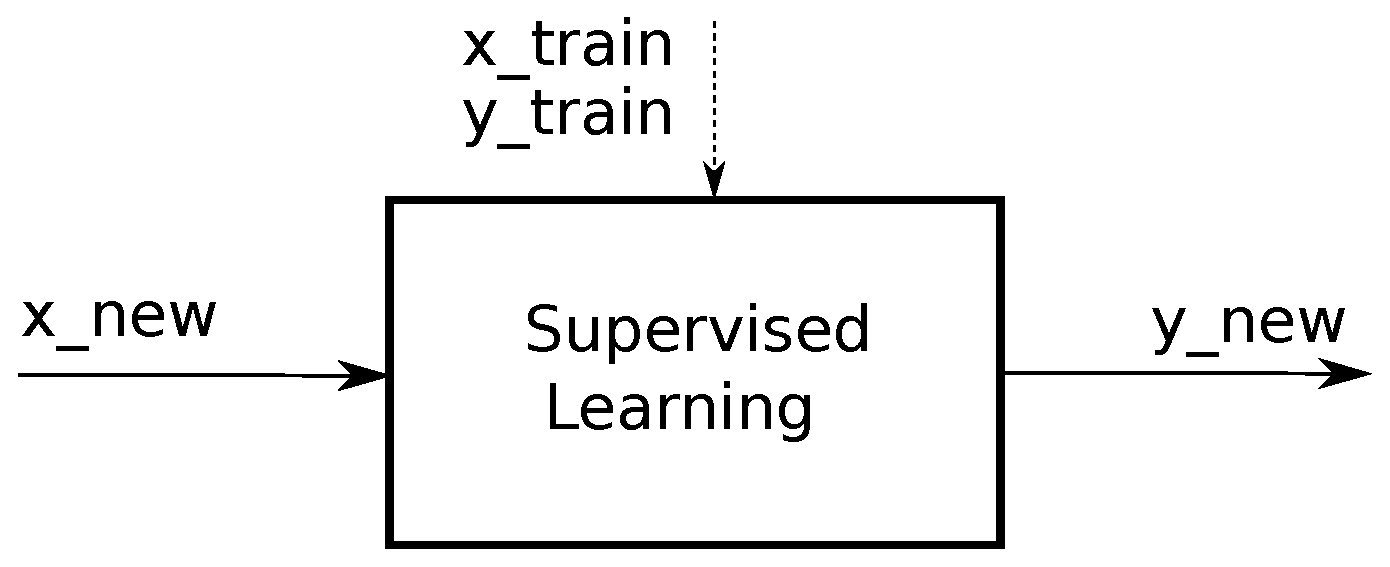
\includegraphics[scale=0.4]{figures/supervisedLearningBlock.eps}
	\end{figure}
	\begin{figure}[ht]
		\centering
		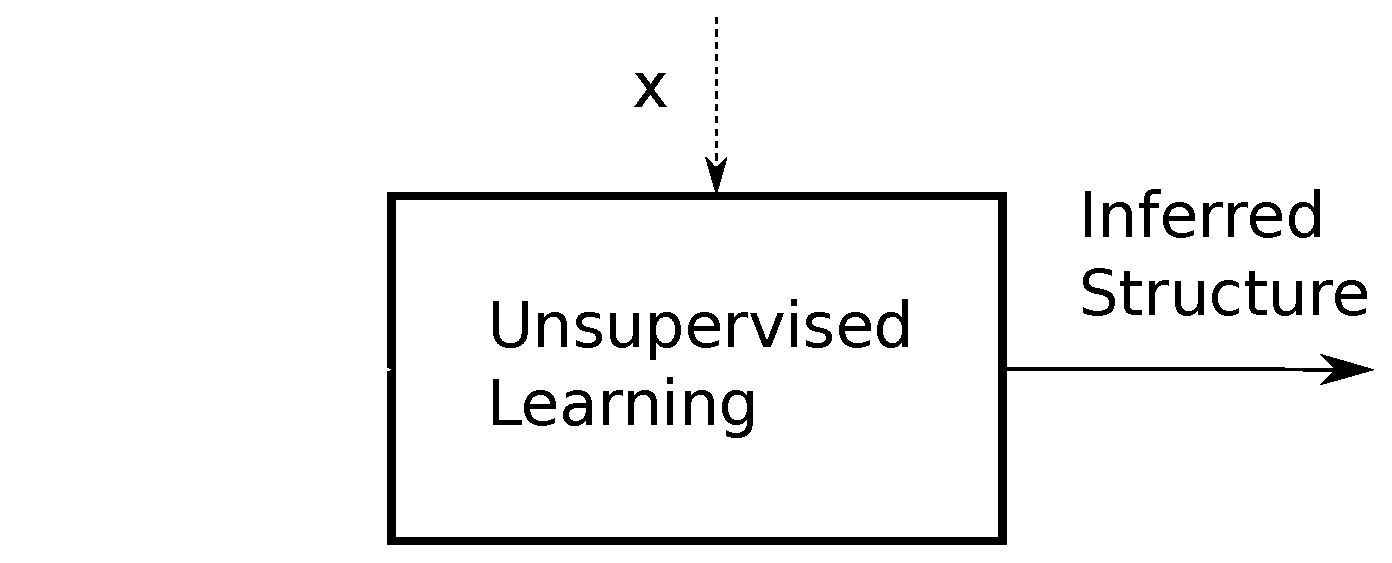
\includegraphics[scale=0.4]{figures/unsupervisedLearningBlock.eps}
	\end{figure}
	\begin{figure}[ht]
	\centering
	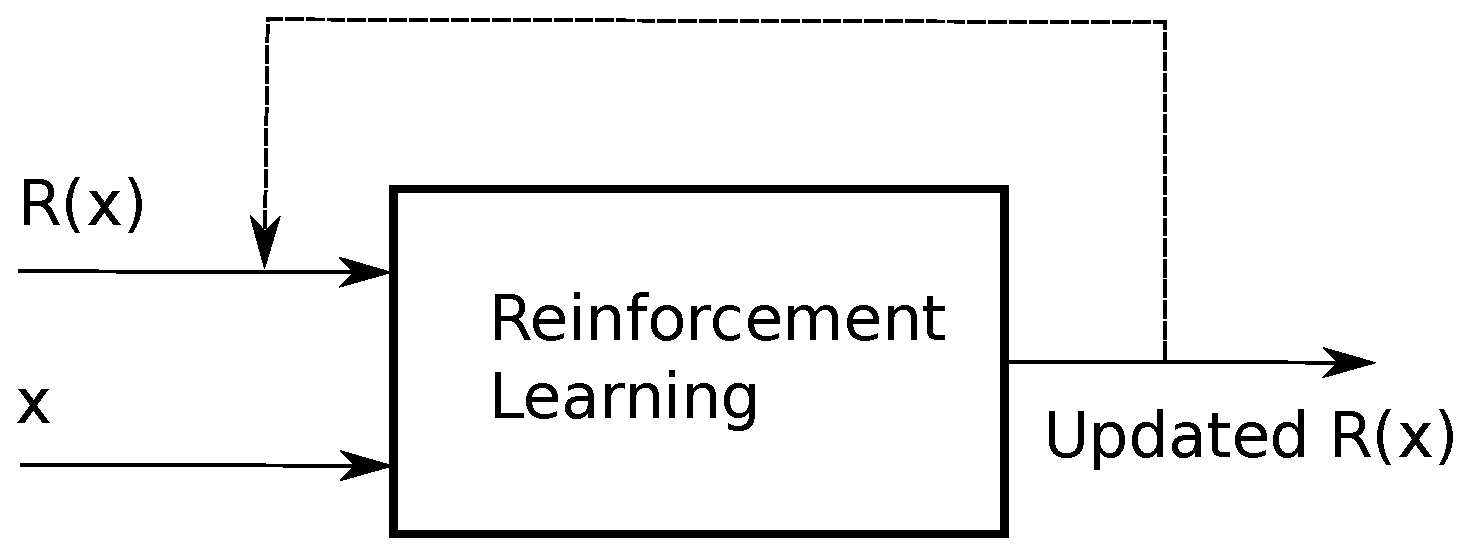
\includegraphics[scale=0.4]{figures/reinforcementLearningBlock.eps}
	\end{figure}
	\begin{figure}[ht]
		\centering
		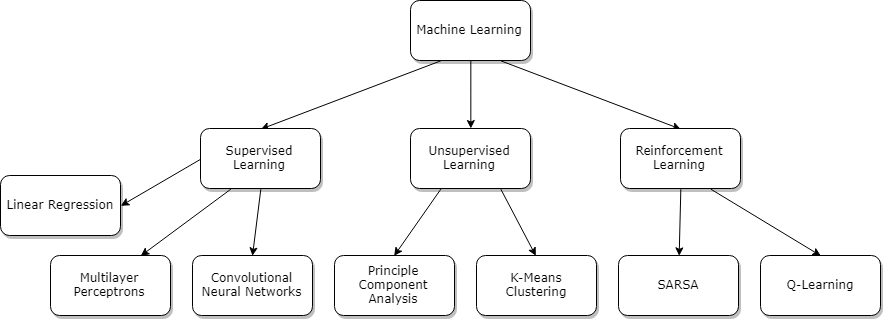
\includegraphics[scale=0.5]{figures/MLdiagram.png}
	\end{figure}
	\par \textbf{\textit{Decide if I want to include actions as part of RL diagram}}
	
	\par Within the CE, concepts from Supervised Learning and Reinforcement Learning are used. As such, the rest of this section will focus on those two categories in more detail. 
	\subsection{Supervised Learning}
	\par As stated before, supervised learning refers to the problem of modeling some sort of relation between two sets of data: an input dataset and a target dataset. This problem is further subdivided into two different types of problems: regression and classification. Regression refers to the modeling of a continuous target. One common example is the modeling of the cost of a house based on its square footage. The other type of problem is classification, which models a discrete target. This is the act of assigning input values to one of a number of different classes. A simple to understand example is determining if someone is likely to renew a magazine based on some collectible information about the person.  
	\par In order to train a model for either problem class, a set of training data similar to the expected input is required, $X_{train}$. In addition to the input set, the resulting target values are needed as well, $Y_{train}$. With this information, the chosen algorithm is trained to understand the nonlinear mapping from input to target. Once the algorithm is trained, it will take $X$ and predict the resulting value of $Y$. There are a wide variety of algorithms that are applied to supervised learning. Relevant algorithms include Linear Regression, Classification and Regression Trees (CART), Multilayer Perceptrons (MLP), and Convolutional Neural Networks (CNN), to name a few. Each of these algorithms requires a different method to update. For this thesis, the relevant classes of supervised learning algorithms are MLP and CART. These will be explained in more detail.
	\par The Classification and Regression Tree (CART) is among the more basic supervised learning techniques still in use today. For each input vector $\vec{x} \in X$, a series of decisions are made based on the values of $\vec{x}$. At each decision, the possible state of the tree is split in two, depending on which value $\vec{x}$ takes. This is more thoroughly described in Algorithm \ref{code:bg_cart}.
	\par 
	\begin{algorithm}[ht]
		\caption{CART Pseudoalgorithm}
		\label{code:bg_cart}
		\begin{algorithmic}[1]
			\Procedure{CART}{}
			\While{$leafNotReached$}
			\State $x = x_{eval} \in X$
			\If {$x > \textit{branchValue}$} Branch right.
			\Else \ Branch left.
			\EndIf
			\EndWhile
			\State \Return $leafValue$ or $leafClass$
			\EndProcedure
		\end{algorithmic}
	\end{algorithm}
	\par One benefit of this algorithm is that it is fairly intuitive, behaving in a way that's similar to how a human might make a decision. It also does not make any underlying assumptions about the underlying data, and doesn't require any parameters. This makes CART an easy method to use. One downside of CART is that it is prone to overfitting. Given $n$ inputs, a tree that splits $n-1$ ways would be capable of 100\% accuracy on the training dataset. However, it would likely underperform on any other data. Because of this, algorithms must be careful to train only until the tree meets the expected specifications in regards to accuracy and other performance metrics. When this issue is taken into account, CARTs act as a good baseline algorithm. This has resulted in them being used in many ensemble-based methods, which use multiple copies of an algorithm to produce results. Ensemble-based methods will be discussed in further detail in Section \ref{bg:advanced_ensemble}.
	
	\par While CART is a simple and useful method, the recent resurgence of Machine Learning as a useful field has been driven by the multilayer perceptron (MLP), also known as a feedforward neural network (FFNN). An MLP is composed of layers of nodes. Each layer is itself composed of nodes, each of which holds a value. The meaning of a node value depends on what type of layer the node belongs to. There are three different types of layers: input layers, hidden layers, and output layers. Input layers are composed of inputs $x_i \in \vec{X}$. Each hidden layer node is a linear combination of all the nodes from the layer before it. How much of each node from the previous layer impacts the current node is defined by a set of weights and biases. After this linear combination, the node applies a nonlinear transform, often called the activation function. Frequently, this transform is used as a squashing function, to limit the outputs to a certain range. The non-linearity is introduced to allow the MLP to represent more complex relationships. Without the activation function, adding additional layers would not result in any increase in representation ability. The output layer takes the values from the last hidden layer and outputs the MLP's prediction of the target value.  
	\par In order to get an effective model, there needs to be some way to evaluate how effective the model is while training it. For an MLP, this is accomplished by using a cost function ($J$), which is a heuristic to evaluate how well the model is performing compared to the ground truth. In the context of a classification problem, a commonly used cost function is cross-entropy, also known as log loss. Cross-entropy is a concept taken from information theory, and represents the average number of bits needed to identify if a sample was taken from distribution $p$ or distribution $q$. By choosing $p=y_{truth}$ and $q=y_{pred}$, cross-entropy can be used as a distance-esque metric. A commonly used cross-entropy based cost function is described in Equation \ref{eq:bg_crossentropy}. This error function is based on a binary classification problem, but can be easily extended to a multi-class problem by combining cost functions for each class.  
	\textbf{\textit{explain each component of the equation after the equation}}
	\begin{align}
		J_{crossEntropy} &= \frac{\sum_N (y_{truth}log(y_{pred}) + (1-y_{truth})log(1-y_{pred}) }{N} \label{eq:bg_crossentropy}
	\end{align}
	\par In the context of a regression problem, a commonly used cost function is mean squared error (MSE). The definition of MSE is given in Equation \ref{eq:bg_mse}. 
	\begin{align}
		J_{MSE} &= \frac{\sum_N (y_{pred}-y_{truth})^2}{N} \label{eq:bg_mse}
	\end{align}
	\par By using these cost functions, a clearer picture about the effectiveness of a model is created. With training reframed as an optimization problem, the simplest solution is to use gradient descent. Upon taking the gradient of the cost function, the resulting value will give an understanding of where the closest maximum of the function is. By updating the weights in the opposite direction of the gradient, the resulting loss value from the updated network will move towards a minimum. This is represented in Equation \ref{eq:bg_gradDescent}, where h represents the value to change the weights W, and J is the Jacobian of the objective function. This method converges well with simpler objective functions, but has the potential to converge slowly, depending on the $\alpha$ parameter and the Jacobian.
	\begin{align}
		h_{gd} &= \alpha J^T W(y_{truth}-y_{pred}) \label{eq:bg_gradDescent}
	\end{align}
	\par Another solution is called the Gauss-Newton method, which is applicable to a sum-of-squares objective function, like $J_{MSE}$. It assumes that the objective function is approximately quadratic near the solution, and uses a first-order Taylor series expansion to approximate the Hessian of the objective function to be $J^TWJ$, where J is the Jacobian of the objective function. This then allows for the weight update procedure to follow Equation \ref{eq:bg_gaussNewton}. This converges much faster than gradient descent for moderately-sized problems, but is applicable to a stricter set of objective functions.
	\begin{align}
		h_{gn} &= (J^TW(y_{truth}-y_{pred}))(J^T WJ)^{-1} \label{eq:bg_gaussNewton}
	\end{align}
	\par The solution that is frequently used (and is the MATLAB default in training a neural network) is the Levenberg-Marquardt method. This is effectively a combination of the two prior optimization problems. It is described in Equation \ref{eq:bg_lm}. 
	\begin{align}
		h_{lm} &= (J^TW(y_{truth}-y_{pred}))(J^T WJ + \lambda \cdot diag(J^T WJ))^{-1} \label{eq:bg_lm}
	\end{align}
	\par $\lambda$ represents the parameter that controls how similar the update is to Gradient Descent, and how similar the update is to Gauss-Newton. A large $\lambda$ represents a similarity to Gradient Descent, and a small $\lambda$ represents a similarity to Gauss-Newton. $\lambda$ is usually initialized to be large, to enable the first updates to be small. If an update increases the objective function, than $\lambda$ is increased. Otherwise, $\lambda$ decreases, moving closer to Gauss-Newton. This is reasonable because as the weights approach the optimal solution, a quadratic assumption is more accurate.
	\par For an algorithm like linear regression, one of these update methods by itself is enough as an update procedure. However, MLPs require a modification of this process. This is due to the multiple layers involved. The process is called Backpropagation. Gradient Descent Backpropagation will be described in Algorithm \ref{alg:bg_gdBackprop}, as it is the simplest to understand. Backpropagation as applied to Levenberg-Marquardt can be found in \cite{lm-backprop}.
	%label{code:bg_backprop}
	\begin{algorithm}
		\caption{Pseudocode for Backpropagation}
		\label{alg:bg_gdBackprop}
		\begin{algorithmic}[1]
			\State Given: training set $X$.
			\Procedure{Backpropagation}{}
			\State Set input activation $a^1=\sigma(X)$
			\For{$l=2$:$L$}
			\State $z^l = w^l a^{l-1} +b^l$
			\State $a^l = \sigma(z^l)$ 
			\EndFor
			\State $\delta^L = \nabla_a C \odot \sigma '(z^L)$
			\For{$l=L-1$:$2$}
			\State $\delta^l = (w^{l+1}\delta^{l+1}) \odot \sigma '(z^l)$
			\EndFor
			\State Output 1: $\frac{\delta C}{\delta w^{l}_{jk}} = a^{l-1}_{k}\delta^{l}_{j}$
			\State Output 2: $\frac{\delta C}{\delta b^{l}_{j}} = \delta^{l}_{j}$
			\EndProcedure
		\end{algorithmic}
	\end{algorithm}
	\par The symbol $\odot$ is the Hadamard Product, which is an element-wise product of two vectors with the same length. $L$ is the number of layers in the MLP. $z^l$ is the weight and bias values at layer $l$, and $a^l$ is $z^l$ passed through the activation function $\sigma(z)$. $\delta^l$ is the error at layer $l$.
	\subsection{Reinforcement Learning}
	\textbf{\textit{Use paulo's RL diagram or something like it}}
	\par While both supervised and unsupervised learning are built on the premise of identifying some form of structure from a given set of data, the goal of Reinforcement learning (RL) is fundamentally different. The core premise of Reinforcement learning is that an agent is trying to learn its environment well enough to know which actions it should take in order to maximize the output of a reward, represented by a function. Each time the agent takes an action, the resulting reward value is is used to update its understanding of the environment.
	\par While there are multiple different ways to pose an RL problem, the one that is most applicable to the problem at hand is the Multi-armed bandit. For an action set, there are multiple reward functions, used as measurements of how well a task was executed. This then becomes an optimization problem for identifying the action set that results in the maximum possible reward. \textit{Another potential model is that of a state-transition problem, modeled as a Markov decision process.} As such, the target problem is changing radio parameters so that optimal performance is achieved in context of the current environmental conditions. There are a wide range of conditions that affect the state-transition model, including the communications channel. This channel is affected by the dynamic geometry of the line-of-sight between the transmitter and receiver, as well as atmospheric and space weather. These complex changing conditions make finding the state-transition model and action-state mapping an intractable pursuit. 
	\par This difficulty is what makes RL a good fit for tackling the problem. The problem then becomes having the agent interact with the environment in an efficient way to find the best possible policy. This also involves balancing the choice of exploration of the environment and exploitation of the information that's been gathered. While the best way to form a policy would be to evaluate the action-value function $Q(s,a)$ at each possible state and action, this becomes infeasible quickly. Instead, the agent should keep exploring policies, with either on-policy or off-policy approaches. On-policy approaches affect the policy that the agent uses to make decisions, while off-policy approaches affect a separate policy from the one that the agent uses to make decisions. Because the target platform is a cognitive engine that adapts to the environment conditions, the focus will be on-policy approaches. 
	\par The model-free method that is relevant to this thesis is Temporal-Difference (TD). This method updates $Q(s,a)$ using the past experiences at each time step. This makes it useful for time-sensitive applications. When used on-policy, it is called State-Action-Reward-State-Action (SARSA), and updates Q by Equation \ref{eq:bg_sarsa}.
	\begin{align}
		Q_{k+1}(s_k,a_k) &= Q_k(s_k,a_k) + \alpha[r + \gamma Q(s_{k+1},a_{k+1})- Q(s_k,a_k)] \label{eq:bg_sarsa}
	\end{align}
	$\alpha$ is the learning rate of the algorithm, r is the reward, $\gamma$ is the discount factor for future rewards, and $s_{k+1}$ and $a_{k+1}$ are the state and action chosen by the current target policy before this update. The value within the brackets is known as TD error, and is the difference between the predicted value of $Q(s_k,a_k)$ and the better prediction of $r + Q(s_{k+1},a_{k+1})$. 
	\par In the context of cognitive radio, only the immediate reward ($\gamma = 0$) is relevant \cite{AIAA_Paper}. In addition, any action can be taken from any state, without the need for planning. This results in a modified SARSA equation, Equation \ref{eq:bg_sarsa2}.
	\begin{align}
		Q_{k+1}(s_k,a_k) &= Q_k(s_k,a_k) + \alpha[r - Q(s_k,a_k)] \label{eq:bg_sarsa2}
	\end{align}
	\par Beyond $Q(s,a)$, a reward function$r = g(s,a)$ and an exploration policy $a = h(s)$ need to be defined before a practical model is complete. In the context of the CE, a multitude of performance functions are relevant to the overall performance of the system. These performance functions may or may not have conflicting responses. The overall result is then represented as a percentage of the maximum performance value. 
	\par In a standard RL system, a knowledge base, or Q-table, is built up. In this Q-table, previous Q-values are mapped to state-action pairs. This table is what gets updated by SARSA.
	
	\par In RL, one of the most important tradeoffs is deciding how much time should be spent exploring the environment versus how much time should be spent exploiting the knowledge already gathered. This is frequently called the Explore-Exploit tradeoff. In context of SARSA, exploring would represent choosing an unvisited action, while exploiting would be choosing an action that has the highest Q value. 
	\par There are many different approaches to tackling the explore-exploit tradeoff. The simplest one is to use an $\epsilon$-greedy algorithm. In this method, an $\epsilon \in (0,1)$ is chosen, which is the probability of choosing a uniformly random action. Otherwise, a greedy action based on the Q-table is chosen. $\epsilon$ is set as a function of time, resulting in more exploration at the beginning of an algorithm, and more exploitation as time goes on and more of the environment is explored. Other methods include value-difference based exploration (VBDE), which changes $\epsilon$ based on TD error, as well as Boltzmann exploration, probability matching, etc. In this work, the classic $\epsilon$-greedy algorithm is used. 
	
	\section{Previous work on NASA SCaN Testbed}
	\par This section first describes the problem that is trying to be solved by the NASA john H. Glenn Research Center (GRC) Space Communications and Navigation (SCaN) Testbed project. With this foundation, the architecture of the cognitive engine (CE) that was developed will be described as well. Finally, the primary goals of the extension that this thesis is focused on will be described.
	
	\textbf{\textit{likely, intro ch and ch2 of paulo's thesis are relevant. Not as much from ch 2 because I don't think that much detail is relevant to this report}}
	\subsection{Problem statement}
	
	\textbf{REPHRASE ALL THIS}
	\par This project is built on top of the SCaN Testbed, an experimental communication system with multiple SDRs used in researching implementation solutions that address issues related to SDR-based communications to and from space. NASA GRC installed the testbed on-board the ISS in 2012, and continues to operate it at GRC. The radios operate at S-band and Ka-band with NASA's satellite relay infrastructure, i.e.,Tracking and Data Relay Satellite System (TDRSS), and operates at S-band in direct communications to ground stations on Earth. The communications to and from the SCAN Testbed provide researches with real-world satellite dynamics between spacecraft and relay satellites or ground stations. Some of these dynamics include time-varying Doppler changes, differences in thermal conditions, interference, range variation, ionospheric effects, and other impairments to propagation.
	\par The SDRs chosen for the SCaN testbed are flight-grade systems, fully compliant with NASA's Space Telecommunications Radio System (STRS) SDR architecture. This architecture provides abstraction interfaces between the radio software and proprietary hardware, allowing for third-party software waveforms and applications to interact with and run on the radio. STRS also provides a library of waveforms available that provide various modulation, coding, framing and data rate options available. 
	\par On top of this platform, solutions such as adaptive communications based on cognitive decision making can be researched, in order to help solve both communication issues on Earth, as well as allowing for the development of space communication systems that will enable space exploration in the near future [131]. SDRs are important in this development, as their flexibility and reconfigurability provides a strong tool. However, SDRs tend to be more complex than traditional fixed-configuration radios. Cognitive radio (CR) systems help reduce the complexity and risk in using these systems. The work that this thesis is extending plays a part in this effort, providing CR algorithm research for SDR systems in space.    
	\subsubsection{REPRHASE}

	\textbf{}\par Three areas have emerged as candidate application areas for CR systems. The different areas are node-to-node communications, system-wide intelligence, and intelligent internetworking. The first application entails the radio-to-radio link between mission spacecraft
	and ground terminal (either through relay or direct-to-ground). Cognitive decision making may improve (increase) throughput across a communication link by consuming otherwise unused designed link margin or mitigating impairments. Algorithms that sense performance
	and understand the entire link capacity could adjust waveform settings to maximize user data and symbol rate by minimizing coding or other overhead. Taking advantage of signifi-cant range changes during a ground station pass or operating at reduced data rates at low
	elevation angles (normally outside the traditional link design) or through weather events offers additional opportunities for additional science data return. Signal recognition among nodes may alleviate missed opportunities due to configuration errors or mitigate unexpected
	interference.
	\par The second application of CR systems is system-wide intelligence where CR systems make operational decisions normally performed by operators or data-intensive aspects not currently done. For example, CR systems could be applied to relay and ground station scheduling, asset utilization (proper asset loading and accommodating mission priority), optimum link configuration and access times, infrastructure fault monitoring, and failure prediction, among others. Many of the applications will help reduce operation oversight (and cost) and help reduce operational complexity due to the large number of possible con-
	figurations. Large data analysis opens a new area to discover  performance and operational benefits from all aspects of data collected including: link performance, platform environment (e.g., radiation, thermal, and mechanical/vibration), asset availability, and system performance.
	%\par Finally, as communications infrastructure becomes more network-based using commercial and international standard protocols, CR systems may benefit the control and data functions of the communications network. Optimizing data throughput according to QoS metrics such as bit error rate, loss packet rate, routing decisions, store-and-forward protocols, and publish-and-subscribe techniques may benefit from cognitive control. Allowing algorithms to learn network behavior, especially small networks with repeatable data flows, may yield throughput and reliability benefits.
	\par One notable aspect regarding CR systems for space is the need for verification or ground testing of all operational conditions before launch. To minimize risk on orbit, missions generally test each mode of operation prior to flight. This helps provide confidence in the onorbit
	operation. Having CR systems make unplanned and potentially unpredictable changes to the flight systems on-orbit will take considerable research and technology demonstrations such as those described in this dissertation.
	
	\par NASA GRC, in Cleveland, Ohio, accepted a proposal entitled “Intelligent MAC protocol for SDR-based satellite communications” with the goal to develop a cognitive engine
	algorithm for future space-based communications systems, with the unique opportunity of experimenting with SCaN Testbed SDR’s. The R\&D team is composed of members from WPI and The Pennsylvania State University, in collaboration with the SCaN team at NASA GRC. Commenced in November 2014, the project is expected to be completed in the May 2017 time frame.
	\par During this collaboration, the team has designed and developed a proof-of-concept of an intelligent MAC protocol to maximize data link performance and to improve the robustness of space communications systems, by using SDRs for low margin data links operating on
	dynamically changing channels, especially at low elevation angles. This protocol’s core is made up of a CE that must be capable of dealing with conflicting multi-objective issues during radio-resource allocation. Adaptation of radio parameters might be required while mitigating channel impairments according to the current channel conditions and/or when meeting new performance requests. Key capabilities to perform cognition are prediction and learning techniques, assisted by third-party databases whenever these are available.
	\par This CE project is aligned with NASA’s Communication and Navigation Systems Roadmap Technology Area 5 [132], which focuses on cognitive radios in space that sense their environment, autonomously determine when there is a problem, attempt to fix it, and learn
	as they operate. This experiment is also one step in the direction of removing communication as a constraint for future missions and their critical phases, and emergency communications to enable safe and efficient human exploration and autonomous robotic space explorations.
	The CE algorithm, as well as simulation and future space-based experiment results will be used to assess the adaptive MAC protocol performance for the on-orbit SDRs, which will help in the design of future MAC protocols and mitigation techniques that can make use of
	the radio flexibility in terms of intelligent radio parameter reconfiguration.
	\par There are four different communication channels between the fixed ground stations at GRC/White Sands, the moving ScaN Testbed SDR on board the ISS, and the TDRSS satellite at a GEO orbit, as illustrated by Figure \textbf{\textit{INCLUDE PICTURE FROM PAULO'S thing}}. Radio parameter reconfiguration might be done during periods of signal fading, especially those happening during low elevation angles of the SCaN Testbed antenna, while tracking the TDRS satellite, or low elevation angles from a GRC ground station antenna, while tracking the ScaN Testbed.
	\par A higher level overview of the proposed CE diagram blocks is shown in Figure 5.2. This basic architecture consists of a gathering observation data, i.e., telemetry data reported
	from the transmitter or measured at the receiver. A predictor uses past information to predict radio parameters values and builds learning in an efficient way in order to keep under control storage memory growth. The decision logic receives the predictions and, based
	on the link performance requirements and resource availability, decides upon the need for adaptation. Future applications and additional sources of information might include thirdparty databases providing atmospheric/space weather data. During radio adaptations, the CE is expected learn the environment behavior by building a model that maps observations into actions, i.e., radio parameter sets, while the channel
	dynamically changes while at a certain channel state. Figure 5.3 illustrates the proposed CE architecture diagram block at a lower level perspective from that shown by Figure 5.2. An initial proof-of-concept ML algorithm implementation of the proposed design shown in Figure 5.2 is a modified version of the classic Reinforcement Learning (RL) algorithm, described in Section 5.2.1. It is specially designed to deal with multi-objective resource allocation in space communications systems. A more complex and autonomous version of this algorithm is proposed in Section 5.3.
	\textbf{Take a lot of the desecription of NASA SCAN stuff from Paolo's section 5.1,almost verbatim}
	\textbf{\textit{include hardware description first}}
	\subsection{ what is the RLNN}
	\subsection{Statement of Work}
	
	\section{Advanced Topics in Machine Learning}
	\subsection{Online Learning and Catastrophic Forgetting}
	\par In supervised learning, there are two different learning paradigms: online learning and offline learning. Offline algorithms assume that there is one set of inputs and outputs to train on, and that once training is complete that there will be no updates to the algorithm. This is contrasted with online algorithms, that update as new data is received. The choice between an offline algorithm and an online algorithm is dependent on the problem that is selected. With a stationary dataset, a single training period can be sufficient. However, if the dataset is nonstationary, there is utility in multiple training periods, which can capture the shifting of the data, also known as concept drift. Because effective space communications systems are dependent on many nonstationary variables, online methods are more suited for this project.
	\par The most basic category of online methods are generalizations of offline methods. In this category, a window of incoming data is collected. Once this window is full, an offline method is trained with this window of data. Then, some number of datapoints is dropped, and the window is filled again. This moving window process is the most straightforward extrapolation of offline algorithms. In the baseline CE, this method is applied to the Levenberg-Marquardt method. The moving-window approach has one major problem that it introduces. The LM algorithm, as well as many first-order offline algorithms (SGD, ADAM, RMSProp, etc.), completely updates the weights completely using the data that is put into it. That means that, as the window moves and drops old datapoints, these old datapoints no longer influence how the model is trained. Because of this, the model will lose the information that was encoded through these datapoints. This is called catastrophic forgetting.  Catastrophic forgetting primarily affects learning in non-stationary environments. If an environment is stationary, the fact that datapoints are no longer used in training has little effect, as the  datapoints replacing them will have similar values. In non-stationary environments, however, the loss of information is more significant. If there is any cyclical nature of the changes, the information will have to be relearned each time.
	\par \textbf{\textit{Include diagram illustrating what the problem with catastrophic forgetting is}}
	\par One way to deal with this is to use a recursive training method. This updates the network based on batches of samples each time, but uses these samples to update an internal state. In this process, there is a forgetting factor built in, allowing for the network to forget past inputs in a more explicit manner than the standard batch-update method. In the following equations, $\varepsilon(h_t) = \sqrt{J(h_t)}$, $P_t$ can be considered the covariance matrix of the weights, $\Omega^T(h_t)$ is a modified gradient for y, allowing for a normalization factor $\rho$ to be added in one weight at a time. This is further described by Ngia and Sjoberg \cite{bg:rlm_establish}. The second row of $\Omega^T(h_t)$ is 0 for all indices where $i\ mod\ nWeights+1 \neq t$, and 1 where $i\ mod\ nWeights+1 = t$. $\alpha$ is the rate of forgetting. 
	\textbf{\textit{REVISIT}}
	\begin{align}
		\Omega^T(h_t) &= \begin{bmatrix}
			&& \nabla_y^T(h_t) && \\ 0 & ... & 1 & ... & 0
		\end{bmatrix} \\
		\Lambda_{T}^{-1} &= \begin{bmatrix}
			1&0\\0&\rho
		\end{bmatrix} \\
		S(h_t) &= \alpha_t\Lambda_t + \Omega^T(w_t)P_{t-1}\Omega(w_t) \\
		P_t &= \frac{1}{\alpha_t}[P_{t-1}-P_{t-1}\Omega(h_t)S^{-1}(h_t)\Omega^T(h_t)P_{t-1}]\\
		h_{t+1} &= h_t + P_t \nabla_y(h_t)\varepsilon(h_t) 
	\end{align}
	\par The update process is split into three substeps, each substep updating a a related aspect of the 
	\subsubsection{Ensemble Learning}\label{bg:advanced_ensemble}
	\par A different approach to deal with Catastrophic Forgetting is to use ensemble training methods. Ensemble methods use a collective of learning algorithms to produce improved results over each individual learning algorithm. In general, ensemble methods use a set of weaker algorithms that are combined with or without some sort of weighting to produce a unified result. In classification problems a weighted majority voting is often used, while in regression problems a weighted median is often used. Frequently, a CART is used as the base algorithm, due to its simple implementation and reasonable performance. Once a base algorithm is chosen, the difference between ensemble implementations is how the ensemble is created and used. For instance, in Adaboost, a series of base learners is trained, with each successive base learner trained in a way that emphasizes points that the previously trained learners have trouble with. This differs from bagging, a different algorithm where each base learner is trained with a different subset of the total training data. These examples are provided simply to show how ensemble learning methods may differ.
	\par The method most relevant to catastrophic forgetting is Learn++.NSE. For each window of samples, Learn++.NSE creates a new learner, trained on the window. It then weights the new learner and existing learners based on how well they work on the training data. In this way, learners that are more applicable to the current environment contribute more.
	\textbf{\textit{PUT ACTUAL PSEUDOALGORITHM HERE, THEN EXPLAIN}}
	\subsection {GANS, and evaluating the utility of them}
	\par One of the major goals of the extension to the Cognitive Engine was to evaluate if the concept of Generative Adversarial Networks, or GANs, was applicable to the project. Like the cognitive engine in its current state, GANs are composed of two neural networks, providing complementary data. In this section, GANS will be described in more detail, as well as their applicability to the CE.  
	\par The primary purpose of a Generative Adversarial Network is to implicitly model some probabilistic data distribution. Prior work has focused primarily on image-based data. Common data distributions to be modeled are MNIST (hand written digits), CIFAR-10 (natural images) and the Toronto Face Dataset (TFD) \cite{gan_overview}. These distributions happen to be all image-based, but there is no explicit need for the data distribution to be an image. 
	\par A GAN is composed of two sub-networks, a Generator($\mathcal{G}$) and a Discriminator($\mathcal{D}$). $\mathcal{G}$ and $\mathcal{D}$ are configured to be in competition. $\mathcal{D}$ is attempting to distinguish between points that are generated by $\mathcal{G}$ and points that are sampled from the true distribution. $\mathcal{D}$ returns a 0 if it thinks the datapoint is not from the true distribution, and a 1 if it thinks the datapoint is. $\mathcal{G}$ is attempting to fool $\mathcal{D}$ into confusing its generated datapoints with the data from the true distribution. Its best case scenario is that $\mathcal{D}$ is only correct around 50\% of the time, as this makes $\mathcal{D}$ only as good as chance.
	\par In a more formal sense, $\mathcal{D}$ can be considered as dealing with a standard classification problem, attempting to classify whether or not a sample it is given is from the real distribution or the artificial one. $\mathcal{G}$ can be considered as dealing with a regression problem, trying to map a random uniform input $U(0,1)$ to the true distribution. Figure \ref{bg:fig_ganDiagram} shows an overview of the GAN architecture. $\mathcal{G}$, modeling a probability distribution, is more difficult than the task of the discriminator, $\mathcal{D}$, classification of incoming data. As such, when the discriminator ceases to improve, it is often frozen, and only $\mathcal{G}$ gets updated. 
	\par The training of a GAN is based on a value function $V(\mathcal{G},\mathcal{D})$ that's dependent on both the generator and the discriminator. Training the GAN accomplishes the following: \textit{THIS NEEDS A BIT MORE}
	\[ \max_\mathcal{D}\min_\mathcal{G} V(\mathcal{G},\mathcal{D}) \] where
	\begin{align}
		V(\mathcal{G},\mathcal{D}) &= E\{p_{real}\}log(\mathcal{D}(x)) + E\{p_{generated}\} log(1-\mathcal{D}(x))
	\end{align}
	\par The first part of $V(\mathcal{G},\mathcal{D})$ represents the log-probability that the discriminator successfully classifies real datapoints as real. The second part represents the log-probability that the discriminator successfully classifies generated datapoints. $\mathcal{D}$ is thus trained by ascending the gradient of $V(\mathcal{G},\mathcal{D})$, and $\mathcal{G}$ is trained by descending a modified version of the gradient. Since $\mathcal{G}$ is only able to affect the probability of $\mathcal{D}$ providing a false positive, it only attempts to minimize this part of $V(\mathcal{G},\mathcal{D})$. This becomes:
	\begin{align}
		\min_\mathcal{G}& E\{p_{generated}\} log(1-\mathcal{D}(x))
	\end{align}
	\par In order to use a non-saturating criterion, the minimization is rearranged to be a maximization, as shown in Equation (\ref{eq:bg_nonsatG}):
	\begin{align}
		\max_\mathcal{G}&E\{p_{generated}\} log(\mathcal{D}(x)) \label{eq:bg_nonsatG} 
	\end{align}
	
	\textit{\textbf{NOT SURE IF SHOULD REFRAME X TO BE G(z) IN THIS OR NOT}}
	\par Beyond the value function, standard gradient-based backpropagation methods are used for updating the networks. Both networks are trained in tandem: a batch of real samples is collected, a batch of generated samples are created, and then the results of feeding these samples through $\mathcal{D}$ are used to update both $\mathcal{D}$ and $\mathcal{G}$.  
	\par \textit{\textbf{Put a diagram here, probably one that I used in powerpoint explanation}}
	\par While GANs are a versatile method for modeling a data distribution, the training process is far from robust. The first issue is that there is no guarantee that the pair of models will converge. Because of the adversarial nature of the network, the convergence requires both models converging with competing objectives.The standard GAN procedure does not have any guarantees that this will happen. Another issue is called mode collapse, and is when $\mathcal{G}$ starts to produce very similar samples for different inputs. This may result in good values for $V(\mathcal{G},\mathcal{D})$, but will only model a specific subset of the real data distribution. A final issue is that the loss value of $\mathcal{D}$ can quickly converge to zero, making there no reliable way to update $\mathcal{G}$. This is called the Vanishing Gradient problem, and is not specific to GANs. 
	\par In practice, there are a couple of approaches that are used to reduce the impact of these issues. One method is to normalize the inputs of each layer by subtracting the input mean and dividing by the input standard deviation. This ensures that inputs of vastly different magnitudes can be represented in a more similar manner. Doing this introduces a "standard deviation" parameter and a "mean" parameter for each node, allowing for the training process to use "denormalized" nodes if it's optimal, without reducing the overall stability.
	\par An approach used to deal with mode collapse is mini-batch discrimination, which adds an input to the discriminator that encodes the distance between a sample in a mini-batch and the other samples. This makes the discriminator able to tell if the generator is producing the same outputs. Another approach, called feature matching, alters the goal of $\mathcal{G}$ to try to match an intermediate activation of $\mathcal{D}$ from real samples with its generated samples. The additional information makes it more able to represent more complex representations. Heuristic averaging, which penalizes network parameters if they stray from a running average of previous values, is a useful approach to aid in making the GAN converge. 
	\par Beyond the heuristic approaches, there have been a few attempts at alternative formulations of GANs that will be more robust. The most prominent approach is the WGAN \cite{bg:wganPaper}. This modifies the cost function of the GAN to use Wasserstein distance, instead of cross-entropy. The details of Wasserstein distance, also known as Earth-Mover distance, are irrelevant to this thesis, and so will be left to further investigation. However, the intuition of Wasserstein distance is that:  
	\begin{itemize}
		\item $P_x$ and $P_y$ are similar to piles of earth. 
		\item $\gamma(x,y)$ is the amount of "mass" that needs to be moved to make $P_x$ into $P_y$.
		\item Wasserstein distance is the "cost" of the optimal transport plan of $\gamma$.
	\end{itemize}
	\par On a surface level, the RLNN has some similarities to the GAN. Like a GAN, the RLNN uses two neural networks working in combination to produce different types of results. However, many of the similarities end here. The performance of the explore and exploit networks are not particularly related, as the performance of one doesn't indicate the performance of the other. Furthermore, neither the explore network nor the exploit network were developed as a classification problem. In order to make these networks fit the GAN structure, there would need to be a restructuring of the RLNN architecture.
	\par Another potential way to use the GAN is in replacement of the explore or exploit network. The Explore network is the model that fits into the standard GAN formation. Indeed, it could be considered to be attempting a similar problem as $\mathcal{G}$. While there would be benefits of replacing the Explore network with a GAN, limitations of the experiment setup prevent doing so. The amount of samples required to properly train a GAN would likely be prohibitive, considering how difficult it is to schedule time to conduct experiments on the space-based platform. As a result of this, the conclusion is that GANs are not directly applicable to the SCaN testbed CE.
	
	\section{LINKS TO CITE}
	\textbf{\textit{As much as possible, use IEEE peer-reviewed things.}}
	https://ai.stanford.edu/~nilsson/MLBOOK.pdf INTRO TO ML \\
	http://www.statsoft.com/Textbook/Classification-and-Regression-Trees CARTS\\
	http://incompleteideas.net/book/bookdraft2017nov5.pdf  RL\\
	https://towardsdatascience.com/machine-learning-fundamentals-via-linear-regression-41a5d11f5220 GRADIENT DESCENT \\
	http://people.duke.edu/~hpgavin/ce281/lm.pdf LEVENBERG MARQUARDT \\
	http://neuralnetworksanddeeplearning.com/chap2.html BACKPROP \\
	http://web.engr.oregonstate.edu/~tgd/publications/mcs-ensembles.pdf ENSEMBLE LEARNING\\
	https://arxiv.org/pdf/1710.07035.pdf GANSTUFF \\
\end{document}